\documentclass[landscape,twocolumn]{article}
\usepackage{biblatex, booktabs, hyperref, graphicx, mathtools, pgfplots, pgfplotstable}
\addbibresource{references.bib}
\pgfplotsset{compat = 1.16}
\pgfplotstableread[col sep=comma]{../Output/results.csv}\results{}
\pgfplotstableread[col sep=comma]{../Output/Naive Bayes.csv}\naivebayes{}
\pgfplotstableread[col sep=comma]{../Output/Logistic Regression.csv}\logisticregression{}
\pgfplotstableread[col sep=comma]{../Output/SVM.csv}\svm{}
\pgfplotstableread[col sep=comma]{../Output/Decision Tree.csv}\decisiontree{}
\pgfplotstableread[col sep=comma]{../Output/Nearest Neighbor.csv}\nearestneighbor{}
\pgfplotstableread[col sep=comma]{../Output/Bagging.csv}\bagging{}
\pgfplotstableread[col sep=comma]{../Output/Ada Boost.csv}\adaboost{}
\title{COMP5318 Assignment 1}
\author{Nicholas Grasevski (ngra5777, 500710654)}
\begin{document}
\maketitle
\begin{abstract}
	In this report several image classifiers are benchmarked against a grayscale image dataset. With the help of some feature engineering, a Support Vector Machine with Radial Basis Function kernel is the highest performing classifier with 89.5\% accuracy on the test set.
\end{abstract}

\section{Introduction}
Object recognition is one of the biggest subfields of computer vision, with many practical applications such as computer aided diagnosis~\cite{doi2007computer}, face detection~\cite{hjelmaas2001face}, Optical Character Recognition~\cite{mori1999optical} and so on.

The current state of the art in object recognition is Convolutional Neural Networks~\cite{iandola2016squeezenet}. The convolutional neural network takes in the raw pixel data and applies several layers of `convolution' transformations, which aggregate nearby pixels into higher order features in a hierarchical fashion. Prior to the prevalence of GPU based neural network training, the previous state of the art was to apply some hand crafted transformations to the input image to extract higher order features~\cite{rybski2010visual}, and then pass the encoded features through a classical machine learning algorithm such as a generalized linear model~\cite{ebrahimzadeh2014efficient}.

The aim of this study is to compare and contrast several different machine learning algorithms when applied to an object detection problem. This should provide insight into their relative ability to capture the information in the data, with the help of some standard hand crafted feature transformations.

\section{Methods}
\begin{figure}[ht]
	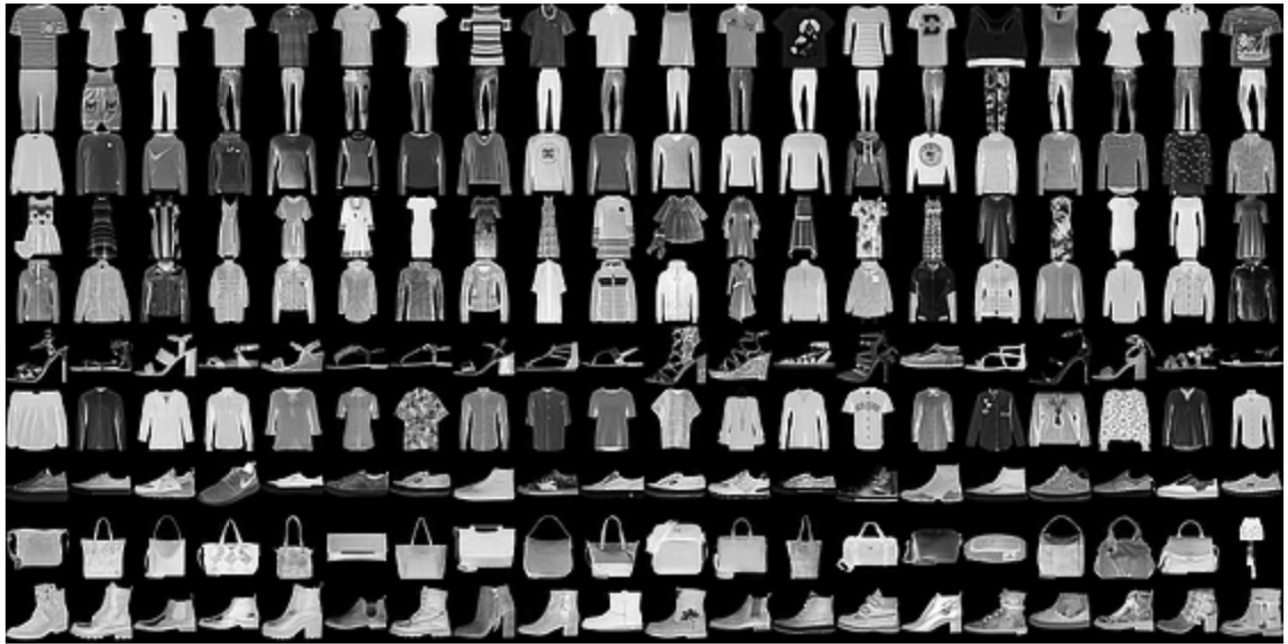
\includegraphics[width=\linewidth]{../Dataset_image}
	\caption{Grayscale $28 \times 28$ images of clothing.}\label{fig:images}
\end{figure}

Several machine learning algorithms were benchmarked against a corpus of $28 \times 28$ grayscale images. Examples of the images can bee seen in figure~\ref{fig:images}. There are 10 classes in total:
\begin{enumerate}
	\item T-shirt/Top
	\item Trouser
	\item Pullover
	\item Dress
	\item Coat
	\item Sandal
	\item Shirt
	\item Sneaker
	\item Bag
	\item Ankle Boot
\end{enumerate}

30,000 of these images are used for training and hyperparameter tuning using 10-fold cross-validation, and 2,000 are used as a hold-out set to evaluate the best classifier according to the cross validation results.

The performance is evaluated primarily based on top-1 accuracy, as defined in equation~\ref{eq:accuracy}:

\begin{equation}
	\label{eq:accuracy}
	\text{Accuracy} = \frac{\text{Number of correct classifications}}{\text{Total number of test examples used}}
\end{equation}

The training and inference time cost of each algorithm is also evaluated. The experiment was performed on a 16-inch 2019 MackBook Pro, with a 2.3GHz 8-Core Intel Core i9 and 32 GB 2667 MHz DDR4 RAM\@.

\subsection{Preprocessing}
The images were preprocessed by first getting the Histogram of Oriented Gradients descriptor, and then passing the descriptor into a Principal Component Analysis.

\subsubsection{Histogram of Oriented Gradients}
\begin{figure}[ht]
	\includegraphics[width=\linewidth]{../Output/hog}
	\caption{Histogram of Oriented Gradients transformation.}\label{fig:hog}
\end{figure}

The input data was preprocessed using a feature descriptor called `Histogram of Oriented Gradients' (HOG)~\cite{dalal2005histograms}. It performs the following steps:
\begin{description}
	\item[Gamma compression] First, the square root of the raw pixel data is taken to reduce the influence of illumination effects.
	\item[Gradient computation] The horizontal and vertical gradients between adjacent pixels are calculated, resulting in each cell having a 2D gradient vector.
	\item[Orientation binning] The orientations of these vectors are discretized, into 8 bins in our case, corresponding to bins from 0 to 180 degrees.
	\item[Cell histogram] These discretized orientations are then aggregated by `cells', which in our case are $4 \times 4$ pixel areas, and collected in a histogram, with each pixel orientation contributing to the histogram according to its magnitude.
	\item[Descriptor blocks] The cells are then grouped into `blocks', which in our case are $3 \times 3$ cell areas, in a sliding window fashion.
	\item[Block normalization] The cells in each block are normalized against one another using the $L_1$ norm in our case.
	\item[Object detection] Finally, the overlapping normalized blocks are flattened into a feature vector, to be fed into a machine learning algorithm.
\end{description}

The HOG descriptor achieves the following tasks:

\begin{description}
	\item[Normalization] The block descriptor normalization provides better invariance to illumination, shadowing, and edge contrast.
	\item[Feature Extraction] The raw pixel data is distilled to a more meaningful representation of the object edges, as can be seen in figure~\ref{fig:hog}.
\end{description}

\subsubsection{Principal Component Analysis}
The output dimension of the HOG descriptor with the aforementioned parameters is 1800 ($\text{9 cells per block} \times \text{25 blocks} \times \text{8 orientations}$) which is more than double the original flattened dimension ($28 \times 28$). This can cause:

\begin{description}
	\item[Slow training] It is computationally intensive to work with these additional dimensions.
	\item[High variance] Having extra artificial dimensions increases the chances of overfitting.
\end{description}

To mitigate these problems, a Principal Component Analysis (PCA)~\cite{wold1987principal} is performed, wherein the input data is factorized into a set of 3 matrices, known as Singular Value Decomposition~\cite{golub1971singular}, as shown in equation~\ref{eq:svd}:

\begin{equation}
	\label{eq:svd}
	\textbf{X}=\textbf{U}\Sigma\textbf{W}^T
\end{equation}

Where $\textbf{X}$ is the input features, $\textbf{U}$ is an n-by-n matrix, $\Sigma$ is an n-by-p rectangular diagonal matrix of positive numbers $\sigma_{\left(k\right)}$, and $\textbf{W}$ is a p-by-p matrix. We can then truncate the $\textbf{W}$ matrix to include only the $L$ largest singular values and their singular vectors, as in equation~\ref{eq:trunc}:

\begin{equation}
	\label{eq:trunc}
	\textbf{T}_L=\textbf{X}\textbf{W}_L
\end{equation}

From this truncated form, we will take the first 128 principal components of the data, thus resulting in a net reduction of the dimension of the original data by a factor of 6.

\subsection{Algorithms}
\begin{table*}
	\begin{tabular}{ccccc}
		\textbf{Name} & \textbf{Train Time} & \textbf{Train Space} & \textbf{Predict Time} & \textbf{Predict Space} \\\toprule
		Logistic Regression & $\mathcal{O}\left(n^2d\right)$ & $\mathcal{O}\left(nd\right) $ & $\mathcal{O}\left(d\right)$ & $\mathcal{O}\left(d\right)$\\
		Naive Bayes & $\mathcal{O}\left(nd\right)$ & $\mathcal{O}\left(d\right)$ & $\mathcal{O}\left(d\right)$ & $\mathcal{O}\left(d\right)$\\
		SVM & $\mathcal{O}\left(n^3d\right)$ & $\mathcal{O}\left(nd\right)$ & $\mathcal{O}\left(nd\right)$ & $\mathcal{O}\left(nd\right)$\\
	\end{tabular}
	\caption{Computational complexity of different algorithms for $n$ features and $d$ dimensions.}\label{tab:algorithms}
\end{table*}

Several different algorithms are applied in turn to the preprocessed data, and a grid of their hyperparameters are explored. A stratified 10-fold cross validation is performed on each hyperparameter combination and the highest scoring (algorithm, hyperparameter) combination is retrained on the entire training set and evaluated on the test set.

In real world applications, time and memory are not infinite and the machine learning is bound by the physical limitations of the hardware. Table~\ref{tab:algorithms} shows the computational complexity of the various algorithms.

\subsubsection{Nearest Neighbor}


\subsubsection{Logistic Regression}
Logistic Regression is a generalization of linear regression to estimate the probability of a given class~\cite{wright1995logistic}. It models a probability by applying the softmax function (or sigmoid in the binary case) to a linear model, as in equation~\ref{eq:lr}:

\begin{equation}
	\label{eq:lr}
	\Pr\left(Y_i=c\right)=\frac{e^{\beta_c \cdot \textbf{X}_i}}{\sum_h{e^{\beta_h \cdot \textbf{X}_i}}}
\end{equation}

Where $Y_i$ is the label of a given sample, $\textbf{X}_i$ is the input vector, and $\beta_c$ is the weight vector from the fitted model for the given class $c$.

It fits a linear decision boundary such that the logistic loss is minimized, as defined in equation~\ref{eq:logisticregression}:

\begin{equation}
	\label{eq:logisticregression}
	L\left(y,p\right)=-\sum{y\log{p}}
\end{equation}

Where $L$ is the loss, $y$ is the ground truth (as a one hot class vector) and $p$ is the predicted probability (as a softmax vector). It is normally trained using batch gradient descent. Although the training for Logistic Regression is slower and more memory intensive than Naive Bayes, the inference complexity is identical, making it a relatively efficient machine learning algorithm.


\subsubsection{Naive Bayes}
Naive Bayes is a generative model that uses Bayes' Theorem to calculate the probability of a given class given the input variables~\cite{rish2001empirical}. The algorithm assumes that the input variables are conditionally independent, ie $\Pr\left(A,B|Y\right)=\Pr\left(A|Y\right)\Pr\left(B|Y\right)$, yielding a closed-form solution to the probability calculation, as can be seen in equation~\ref{eq:naivebayes}:

\begin{equation}
	\label{eq:naivebayes}
	\Pr\left(C_k|x_1,\ldots,x_n\right)=\frac{1}{Z}\Pr\left(C_k\right)\prod_{i=1}^n{\Pr\left(x_i|C_k\right)}
\end{equation}

For class $C$, where the evidence $Z=\Pr\left(\textbf{X}\right)=\sum_k{\Pr\left(C_k\right)\Pr\left(\textbf{x}|C_k\right)}$ is a scaling factor dependent only on $x_1,\ldots,x_n$, that is, a constant if the values of the feature variables are known.

This simple formulation makes training Naive Bayes very computationally efficient and also easily parallelizable, thanks to the conditional independence assumption. However, the assumption rarely holds in practise, leading to poor performance compared to more sophisticated techniques.

\subsubsection{Decision Tree}
\subsubsection{Bagging}
\subsubsection{Ada Boost}

\subsubsection{Support Vector Machine}
Support Vector Machine is a supervised learning algorithm which produces a non-probabilistic classifier, attempting to separate the classes by a set of hyperplanes. It can be used as a linear classifier, or for any nonlinear `kernel' satisfying Mercer's condition~\cite{noble2006support}. This gives it more predictive power compared to Naive Bayes (which can only predict based on statistically independent variables) and Logistic Regression (which can only predict a linear decision boundary). However the additional power afforded by nonlinearity comes at a cost, as the resultant optimization problem must be solved using a quadratic programming algorithm such as coordinate descent, which typically has cubic time complexity. Furthermore the inference time can be an order of magnitude slower compared to Naive Bayes and Logistic Regression. More than one weight vector is required, and the number of weight vectors required is proportional to the size of the input data.

\section{Experiments and results}
\begin{table}
	\pgfplotstabletypeset[
	columns={name,score,time_seconds},
	columns/name/.style={string type,column name=Model},
	columns/score/.style={multiply by=100,column name={CV Acc\%}},
	columns/time_seconds/.style={column name={Training Time (s)}},
	every head row/.style={after row=\toprule},
	]{\results}
	\caption{Comparison of machine learning algorithms.}\label{tab:results}
\end{table}

\begin{figure}
	\begin{tikzpicture}
		\begin{axis}[
			title={CV Accuracy},
			ybar, nodes near coords,
			xlabel={Model},
			xtick=data,
			xticklabels from table={\results}{name},
			x tick label style={rotate=90,anchor=east},
			ylabel={CV Accuracy (\%)}
			]
			\addplot table[x expr=\coordindex, y expr=100*\thisrow{score}]{\results};
		\end{axis}
	\end{tikzpicture}
	\caption{Comparison of cross validation accuracy.}\label{fig:accuracy}
\end{figure}

\begin{figure}
	\begin{tikzpicture}
		\begin{axis}[
			title={Training Time},
			ybar, nodes near coords,
			xlabel={Model},
			xtick=data,
			xticklabels from table={\results}{name},
			x tick label style={rotate=90,anchor=east},
			ylabel={Training Time (s)}
			]
			\addplot table[x expr=\coordindex, y expr=\thisrow{time_seconds}]{\results};
		\end{axis}
	\end{tikzpicture}
	\caption{Comparison of cross validation accuracy.}\label{fig:time}
\end{figure}

As can be seen in table~\ref{tab:results}, there is a tradeoff between training speed and accuracy. Naive Bayes is by far the fastest to train, but does not achieve great accuracy. SVM is the slowest to train, but is highly accurate by comparison. Logistic Regression is slow to train, but notably has similar inference speed to Naive Bayes, due to the same algorithmic complexity during inference.

Although naive bayes has the lowest accuracy, it is still decent. This is testament to the effectiveness of the feature engineering and preprocessing that was done to normalize the data and extract meaningful independent features.


\subsubsection{Nearest Neighbor}
\begin{table*}
	\pgfplotstabletypeset[
	columns={param_n_neighbors,param_p,mean_test_score,std_test_score,mean_fit_time,std_fit_time,mean_score_time,std_score_time},
	columns/param_n_neighbors/.style={column name=k},
	columns/param_p/.style={column name=p},
	columns/mean_test_score/.style={multiply by=100,column name={Acc\%}},
	columns/std_test_score/.style={multiply by=100,column name=STD},
	columns/mean_fit_time/.style={column name={Fit Time (s)}},
	columns/std_fit_time/.style={column name=STD},
	columns/mean_score_time/.style={column name={Score Time (s)}},
	columns/std_score_time/.style={column name=STD},
	every head row/.style={after row=\toprule},
	]{\nearestneighbor}
	\caption{Nearest Neighbor cross validation results.}\label{tab:nearestneighbor}
\end{table*}


\subsubsection{Logistic Regression}
\begin{table*}
	\pgfplotstabletypeset[
	columns={param_C,param_penalty,mean_test_score,std_test_score,mean_fit_time,std_fit_time,mean_score_time,std_score_time},
	columns/param_C/.style={column name=C},
	columns/param_penalty/.style={string type,column name=Penalty},
	columns/mean_test_score/.style={multiply by=100,column name={Acc\%}},
	columns/std_test_score/.style={multiply by=100,column name=STD},
	columns/mean_fit_time/.style={column name={Fit Time (s)}},
	columns/std_fit_time/.style={column name=STD},
	columns/mean_score_time/.style={column name={Score Time (s)}},
	columns/std_score_time/.style={column name=STD},
	every head row/.style={after row=\toprule},
	]{\logisticregression}
	\caption{Logistic Regression cross validation results.}\label{tab:logisticregression}
\end{table*}

As per table~\ref{tab:logisticregression}, two parameters were tuned for logistic regression:

\begin{description}
	\item[C] Inverse of regularization strength. A regularization strength of 1 (corresponding to the uniform prior) performed best, making a good balance between bias and variance.
	\item[Penalty] What type of regularization to use. $L_1$ and $L_2$ regularization were both attempted (corresponding to assumptions of laplacian and gaussian noise respectively), with $L_2$ performing consistently better. Perhaps the images naturally had some gaussian noise, allowing the $L_2$ penalty to account for that noise more effectively than the $L_1$ penalty. It is also conceivable that the sparseness enforced by the $L_1$ penalty is undesirable as the input data is continuous numerical data, so taking individual points (pixel groups in this case, due to the HOG transform) and discarding the surrounding context may cause overfitting when generalizing to the test data.
\end{description}


\subsubsection{Naive Bayes}
\begin{table*}
	\pgfplotstabletypeset[
	columns={mean_test_score,std_test_score,mean_fit_time,std_fit_time,mean_score_time,std_score_time},
	columns/mean_test_score/.style={multiply by=100,column name={Acc\%}},
	columns/std_test_score/.style={multiply by=100,column name=STD},
	columns/mean_fit_time/.style={column name={Fit Time (s)}},
	columns/std_fit_time/.style={column name=STD},
	columns/mean_score_time/.style={column name={Score Time (s)}},
	columns/std_score_time/.style={column name=STD},
	every head row/.style={after row=\toprule},
	]{\naivebayes}
	\caption{Naive Bayes cross validation results.}\label{tab:naivebayes}
\end{table*}

Being a simple algorithm, no hyperparameters were tuned for Naive Bayes. As per table~\ref{tab:naivebayes}, Both training and inference time were infinitesimal, thanks to the linear time complexity of the algorithm.


\subsubsection{Decision Tree}
\begin{table*}
	\pgfplotstabletypeset[
	columns={param_ccp_alpha,param_criterion,mean_test_score,std_test_score,mean_fit_time,std_fit_time,mean_score_time,std_score_time},
	columns/param_ccp_alpha/.style={column name={$\alpha$}},
	columns/param_criterion/.style={string type,column name=Criterion},
	columns/param_splitter/.style={string type,column name=Splitter},
	columns/mean_test_score/.style={multiply by=100,column name={Acc\%}},
	columns/std_test_score/.style={multiply by=100,column name=STD},
	columns/mean_fit_time/.style={column name={Fit Time (s)}},
	columns/std_fit_time/.style={column name=STD},
	columns/mean_score_time/.style={column name={Score Time (s)}},
	columns/std_score_time/.style={column name=STD},
	every head row/.style={after row=\toprule},
	]{\decisiontree}
	\caption{Decision Tree cross validation results.}\label{tab:decisiontree}
\end{table*}


\subsubsection{Bagging}
\begin{table*}
	\pgfplotstabletypeset[
	columns={param_max_samples,param_n_estimators,mean_test_score,std_test_score,mean_fit_time,std_fit_time,mean_score_time,std_score_time},
	columns/param_max_samples/.style={multiply by=100,column name={Sample\%}},
	columns/param_n_estimators/.style={string type,column name=n},
	columns/mean_test_score/.style={multiply by=100,column name={Acc\%}},
	columns/std_test_score/.style={multiply by=100,column name=STD},
	columns/mean_fit_time/.style={column name={Fit Time (s)}},
	columns/std_fit_time/.style={column name=STD},
	columns/mean_score_time/.style={column name={Score Time (s)}},
	columns/std_score_time/.style={column name=STD},
	every head row/.style={after row=\toprule},
	]{\bagging}
	\caption{Bagging cross validation results.}\label{tab:bagging}
\end{table*}


\subsubsection{Ada Boost}
\begin{table*}
	\pgfplotstabletypeset[
	columns={param_learning_rate,param_n_estimators,mean_test_score,std_test_score,mean_fit_time,std_fit_time,mean_score_time,std_score_time},
	columns/param_learning_rate/.style={multiply by=100,column name={$\lambda$}},
	columns/param_n_estimators/.style={string type,column name=n},
	columns/mean_test_score/.style={multiply by=100,column name={Acc\%}},
	columns/std_test_score/.style={multiply by=100,column name=STD},
	columns/mean_fit_time/.style={column name={Fit Time (s)}},
	columns/std_fit_time/.style={column name=STD},
	columns/mean_score_time/.style={column name={Score Time (s)}},
	columns/std_score_time/.style={column name=STD},
	every head row/.style={after row=\toprule},
	]{\adaboost}
	\caption{Ada Boost cross validation results.}\label{tab:adaboost}
\end{table*}


\subsubsection{Support Vector Machine}
\begin{table*}
	\pgfplotstabletypeset[
	columns={param_C,param_kernel,mean_test_score,std_test_score,mean_fit_time,std_fit_time,mean_score_time,std_score_time},
	columns/param_C/.style={column name=C},
	columns/param_kernel/.style={string type,column name=Kernel},
	columns/mean_test_score/.style={multiply by=100,column name={Acc\%}},
	columns/std_test_score/.style={multiply by=100,column name=STD},
	columns/mean_fit_time/.style={column name={Fit Time (s)}},
	columns/std_fit_time/.style={column name=STD},
	columns/mean_score_time/.style={column name={Score Time (s)}},
	columns/std_score_time/.style={column name=STD},
	every head row/.style={after row=\toprule},
	]{\svm}
	\caption{SVM cross validation results.}\label{tab:svm}
\end{table*}

As per table~\ref{tab:svm}, two main hyperparameters were tested for SVM:\@

\begin{description}
	\item[C] Inverse of regularization strength. In this case, a regularization strength of 10 performed marginally better than other settings.
	\item[Kernel] Which kernel type to use. The Radial Basis Function performed the best. This makes sense because intuitively it is grouping together images which have edges in similar locations, whereas the linear kernel (ie no kernel) would mostly classify based on the overall contrast of each group of pixels in the image, with no consideration for the proximity of said groups of pixels. The polynomial kernel also performed well, the default setting is degree 3, perhaps degree 2 could provide better results. The sigmoid kernel performed worst.
\end{description}

\section{Conclusion}
Out of the algorithms applied, Support Vector Machine achieved the highest accuracy at the expense of a relatively long training time. Naive Bayes was by far the fastest in both training and inference, due to the efficient time complexity of the algorithm. Further improvements would be to consider convolutional neural networks in order to automatically extract similar features to the HOG descriptor via backpropagation and stochastic gradient descent. Furthermore, GPU acceleration could be utilized to achieve fast training and inference by parallelizing the pixel-wise operations which are very common in computer vision.

\printbibliography\appendix
\section{Running the code}
\begin{description}
	\item[Dependencies] \texttt{pip3 install h5py pandas scikit-image scikit-learn}
	\item[Usage] Run the steps in the notebook sequentially to get the tuning and evaluation results.
\end{description}

Detailed cross validation results will be written as csv files to \texttt{Output} for each respective classifier, along with the final predictions as \texttt{Output/predicted\_labels.h5}. Note that the \texttt{ALGORITHMS} parameter can be modified at will to change the grid search process, for example to speed up the runtime of the script by excluding certain algorithms or hyperparameter combinations.

\end{document}
